
\documentclass[12pt]{article}
\usepackage{amsmath, amssymb}
\DeclareMathOperator{\Tr}{Tr}
\usepackage{bbold}
\usepackage{graphicx}
\usepackage{hyperref}
\graphicspath{{images/}}
\usepackage[top = 2.5cm, bottom = 2.5cm, left = 2.5cm, right = 2.5cm]{geometry}
\usepackage{natbib} % To cite
\usepackage[ruled,vlined]{algorithm2e}
\title{Coalescence manuscript}

\begin{document}
	\maketitle
	\section{Introduction}
	
    	Microbial communities are widespread throughout our planet \citep{Fierer2006}, from the deep ocean to the human gut, and play a critical role in natural processes ranging from animal development and host health \citep{Huttenhower2012, McFall-Ngai2013} to biogeochemical cycles \citep{Falkowski2008}. These communities are very complex, often harbouring hundreds of species \citep{Gilbert2014}, making them hard to characterize. Recently, DNA sequencing has allowed a high-resolution mapping of these consortia, opening a niche for ambitious theorists and experimentalists to collaboratively disentangle the complexity of these systems \citep{Marsland2019, Goldford2018, Goyal2018, Friedman2017, Costello2012, Vila2019, Estrela2020, Coyte2021}. Despite thorough explorations, the mechanisms responsible for the assembly of microbiome communities have only begun to be revealed. \par
    	Unlike in the macroscopic world, entire microbial communities often suffer displacements to different regions, where they encounter other communities. The process by which two or more communities that were previously separated join and reassemble into a new community has been termed community coalescence \citep{Rillig2015}. This type of event  happens repeatedly in microbiomes due to abiotic (wind, tides or river flow), biotic (animal courtship, parent-offspring interactions or leaves falling), and anthropogenic (industrial anaerobic digestion, agriculture, between-human contact) factors \citep{Luo2020, Vass2021, Castledine2020}. Notwithstanding the frequency and importance of microbial community coalescence, the mechanisms responsible for the community structure and function resulting from coalescence events remain poorly understood \citep{Rillig2016b}.\par
    	Early mathematical models of community-community invasion revealed that when two communities previously separated by a barrier merge due to its removal, asymmetrical dominance of one community over the other one is likely to occur \citep{Gilpin1994, Toquenaga1997}. As an explanation for this observation, it was argued that, because communities have been assembled through a history of competitive exclusion, they are likely to compete with each other as coordinated entities, rather than as a random collection of species. This result also stems from later theoretical work, where consumer-resource models are used to show that in a microbial community coalescence event, the winning community will be that which is capable of simultaneously depleting all resources more efficiently. \citep{Tikhonov2016, Tikhonov2017}.  Overall, these findings suggest that communities arising from competitive species sorting experiment a certain level of cohesiveness that makes them less vulnerable to invasions by other communities.\par 
    	Similar results arise from coalescence experiments with methanogenic communities \citep{Sierocinski2017}, where it is reported that during a coalescence event, multiple taxa from the community with the most efficient resource use act as cohesive units and are selected together (ecological co-selection). Further experimental evidence of co-selection in community coalescence has been reported in \citet{Lu2018}, where it was shown that the invasion success of a given taxon is determined by its community members. The microbial communities used in these experiments are characterized by complex cross-feeding interactions \citep{Hansen2007, Lawrence2012, Embree2015}, where the metabolic by-products of one species are substrates for others.
    	Furthermore, a densely connected metabolic network of cross-feeding relationships has been recognized as one of the mechanisms allowing the stable coexistence of many species in microbiome communities. \citep{Goldford2018}. Recently, it has been pointed out that the type and strength of the interactions present in microbial communities is a factor that might affect the outcome of community coalescence \citep{Castledine2020}. However, theoretical explorations of community-community invasions up to date have considered competition for abiotic resources as the only ecological force driving the outcome of these events. It is then natural to ask what would be the  effect of other types of interactions, namely, mutualism, in determining the result of community-community encounters. \par
    	Here we use a consumer resource model that includes metabolic cross-feeding to study the combined role of mutualistic and competitive interactions in community assembly and community coalescence simulations. First, we use this model to assemble microbial communities spanning a broad range in the competitive-cooperative spectrum. Second, we perform pairwise coalescence experiments between the assembled communities. Third, we \par\\
    	
	\section{Theory}
	    Here, we motivate and present the model used for the simulations and explain the assumptions we make. Next, we propose metrics for the levels of competition and mutualism expressed within the framework of the model.
    	\subsection{Model}\label{model}
    	
        	In order to simulate communities with cross-feeding interactions, I use a consumer-resource model adapted from the work of \cite{Marsland2019}. Consider an environment with $ m $ resources present in different concentrations $ R_{j} $, where $ j \in \{1 \dots m\} $. Let now $ n_{\alpha} $ denote the abundance of each bacterial strain $ \alpha $  present in the environment, $ \text{ where } \alpha \in \{1 \dots s\} $. Each species is uniquely characterized by the metabolic strategy it uses to harvest resources. Additionally, all species share a core metabolism so that a fraction each consumed resource is released in the form of other resources to the environment. If we now allow the dynamics of this system to unfold, the concentration of each metabolite $ R_j $ determines the dynamics of the abundances $ n_\alpha$ of each species, which harvest resources according to their metabolic strategies and secrete by-products through the metabolic network. The change in species abundances translate into changes in the total supply and demand of resources. In turn, resource concentrations $ R_j $ are depleted until equilibrium is reached. \par \\
        	The following assumptions are made on the above model: (1) all resources contain the same amount of energy (taken to be 1 for simplicity), (2) a type I functional response, (3) a binary matrix of consumer preferences and (4) a complex environment where all resources are externally supplied in equal amount.\\
        	These assumptions correspond to the following equations for the change in consumer biomass and resource abundance with time
    		\begin{align}
    		    \frac{dn_{\alpha}}{dt} &= g_{\alpha}n_{\alpha}\left((1-l)\sum_jc_{\alpha j}R_j - z_{\alpha}\right)\label{model_pop}\\
    		    \frac{dR_{j}}{dt} &= \kappa_j - \tau^{-1}_jR_j - \sum_{\alpha}n_{\alpha}c_{\alpha j}R_j + l\sum_{\alpha k}n_{\alpha}D_{kj}c_{\alpha k}R_k\label{model_rec}
    		\end{align}
        	In equation \ref{model_pop}, the growth of species $ {\alpha} $ is determined by the resources it harvests, which in turn depends on the resource concentration $ R_j $, and whether or not the species $ {\alpha} $ consumes resource $ j $ ($ c_{{\alpha}j} = 1 \text{ or } c_{{\alpha}j} = 0 $, respectively). However, not all the harvested resources contribute to growth. A fraction of them, $  l $, leak back to the environment as metabolic by-products. Additionally, species $ {\alpha} $ retain some of the harvest for its living maintenance cost $ z_{\alpha} $. For simplicity, we assume this cost to be random:
        	\begin{equation}\label{cost}
        	    z_{\alpha} = \chi_0\sum_j c_{\alpha j} (1 + \epsilon)
        	\end{equation}
        	Here, $\chi_0$ is the average cost of being able to consume a given metabolite, the summation represents the number of resources that species $\alpha$ is able to process, and $\epsilon$ is a random fluctuation sampled from a truncated normal distribution (to ensure that $z_{\alpha} > 0$). The effect of the cost function in equation \ref{cost} is to ensure that neither generalists nor specialists are systematically favoured during the community assembly see section \ref{cost_tradeoff}.\\
        	The remaining resources after subtracting secretions and maintenance are transformed into biomass through $ g_{\alpha} $, a proportionality constant relating energy to abundance of strain $ {\alpha} $. \par 
        	In equation \ref{model_rec}, $ \kappa_j $ and $ \tau_j^{-1} $ encode the external dynamics of the resources; they are the supply and dilution rate of resource  $ j $, respectively. The leakage fraction is $ l $, ($ 0 < l < 1 $), and $ D_{jk} $ encodes the metabolic matrix. Each element of $ D_{jk} $ represents the leaked energy of resource $ j $ that is transformed into resource $ k $. Note that by definition, $ D $ is a row stochastic matrix, i.e., its rows sum to 1. Note that the equations of the model are expressed in index notation; the expressions in matrix form can be found in section \ref{matrix_representations}\par
        	
        \subsection{Competition and facilitation metrics}\label{metrics}
        	
        	In this framework, competition for resources exists because the metabolic preferences vectors of the species in the community will have, in general, some level of overlap. We define intrinsic competition between  a pair of species $(\alpha, \beta)$ as the level of overlap between their metabolic preferences, independently from the environment in which they are. We choose to calculate their metabolic overlap by counting the number of common preferences. Since these are binary, taking the scalar product of the two preference vectors yields the number of common elements between them
        	\begin{equation}
        	    (C_i)_{\alpha \beta} = \sum_kc_{\alpha k}c_{\beta k}
        	\end{equation}
        	The intrinsic competition becomes effective competition when we consider the environment experienced by the consumers. For example, if two species consume metabolite 1, but this metabolite is not supplied, there is intrinsic competition for 1, but not effective competition. The resources available in the environment for a species to consume have two possible origins; abiotic (when they come from the external supply $\kappa$), and biotic (if they have been leaked by fellow species through $l$ and $D$). Depending on the provenance of the resources, the effective competition (to which we will refer, for short, as 'competition' from now on) between any given pair of species can be abiotic, or biotic, and is calculated differently.\par \\
        	When resources come from the external supply, the competition for each resource is weighted by the normalized resource supply $ \tilde{\kappa} = \vec{\kappa}/\text{max}(\vec{\kappa})$. The strength of these interactions is given by $1 - l$, the fraction of resources that are consumed abiotically. Thus, the overall abiotic competition $C_a$ between the species pair $(\alpha, \beta)$ is
        	\begin{equation}\label{abiotic}
        		(C_a)_{\alpha\beta} = (1-l) \sum_k \tilde{\kappa}_kc_{\alpha k}c_{\beta k}
        	\end{equation}
            
            Now consider the biotic competition $C_b$ between species $\alpha$ and $\beta$ for resource $k$, that they have previously leaked to the environment by consuming resource $j$. There will only be biotic competition for $k$ when the following two conditions hold: 1) $\alpha$ or $\beta$ consume metabolite $j$ and leak a fraction of it in the form of metabolite $k$; 2) $\alpha$ and $\beta$ consume $k$. Mathematically, the above conditions take the form
            \begin{equation}\label{little_biotic_term}
                (C_b)^{k\rightarrow j}_{\alpha \beta} \propto D_{jk}\left(c_{\alpha j} + c_{\beta j}\right)c_{\alpha k}c_{\beta k}
            \end{equation}
            The strength of biotic competitive interactions is given by $l$; the fraction of resources present in the environment due to biotic activity that is available for re-consumption (see section \ref{infinite_cycles} for a detailed discussion). Thus, the total biotic competition between the species pair $(\alpha, \beta)$ can be expressed as the sum of the terms that arise from expression \ref{little_biotic_term} when spanning the full resource space, weighted $l$
            \begin{equation}\label{biotic}
        		(C_b)_{\alpha\beta} = l \sum_{jk} \tilde{\kappa}_jD_{jk}\left(c_{\alpha j} + c_{\beta j}\right)c_{\alpha k}c_{\beta k}
        	\end{equation}
        	Note that the leaked resources ultimately come from supplied resources, so we account for possible differences in resource supply rate with the factor $\tilde{\kappa}_j$. After these considerations, we can write the total community competition matrix as \par
            \begin{equation}\label{competition}
                C_T = C_a + C_b
            \end{equation}
            
            Facilitation links form when a species secretes by-products that are used by another species. Therefore, the facilitation of species $\alpha$ to $\beta$ of metabolite $k$, due to the consumption of metabolite $j$, will be non-zero when 1) species $\alpha$ produces $k$ as a by-product when consuming $j$, and 2) species $\beta$ consumes $k$. Analogously to the case of biotic competition, the strength of these interactions is also given by $l$ and a factor $\tilde{\kappa}_j$ is also needed. Thus, the total facilitation of species $\alpha\rightarrow \beta$ will be
            \begin{equation}\label{facilitation}
                F_{\alpha \beta} = l\sum_{jk} \tilde{\kappa}_jc_{\alpha j}D_{jk}c_{\beta k}
            \end{equation}
            Note that facilitation is directional, which implies that the community facilitation matrix $F$ is not symmetric. However, the community competition matrix $C$ is symmetric, since competition is not directional.\par\\
            Averaging the matrices of equations \ref{competition} and \ref{facilitation} yields a proxy of the overall community competition and facilitation levels. The matrix diagonals are left out of the mean calculation, since we are only interested in inter-specific competition and facilitation. Additionally, we only consider the upper diagonal elements of the symmetric competition matrix. With this constrains, the community-level competition and facilitation measures are, respectively
            \begin{equation}
                \mathcal{C} =  \langle C_T_{\alpha \beta} \rangle_{\alpha > \beta}\qquad \qquad \qquad \mathcal{F} =  \langle F_{\alpha \beta} \rangle_{\alpha \neq \beta}
            \end{equation}

    \section{Workflow}
    
        Following the explanation of the theory supporting this work, we proceed to the analysis. First, we sample the consumer preferences and metabolic parameters from random distributions. We impose specific constraints to this distributions in order to broaden the range of competition and facilitation levels in the communities. Second, we simulate all instances of community assembly. Next, we perform community coalescence simulations between random pairs of communities. Finally, we analyse the species abundance in the mix and compare it to the original species abundances in each species. We try to explain the differences with the interactions between community members. The parameter values used in the simulations performed here can be found in section \ref{parameter_values}.
        \begin{figure}[t]
            \centering
            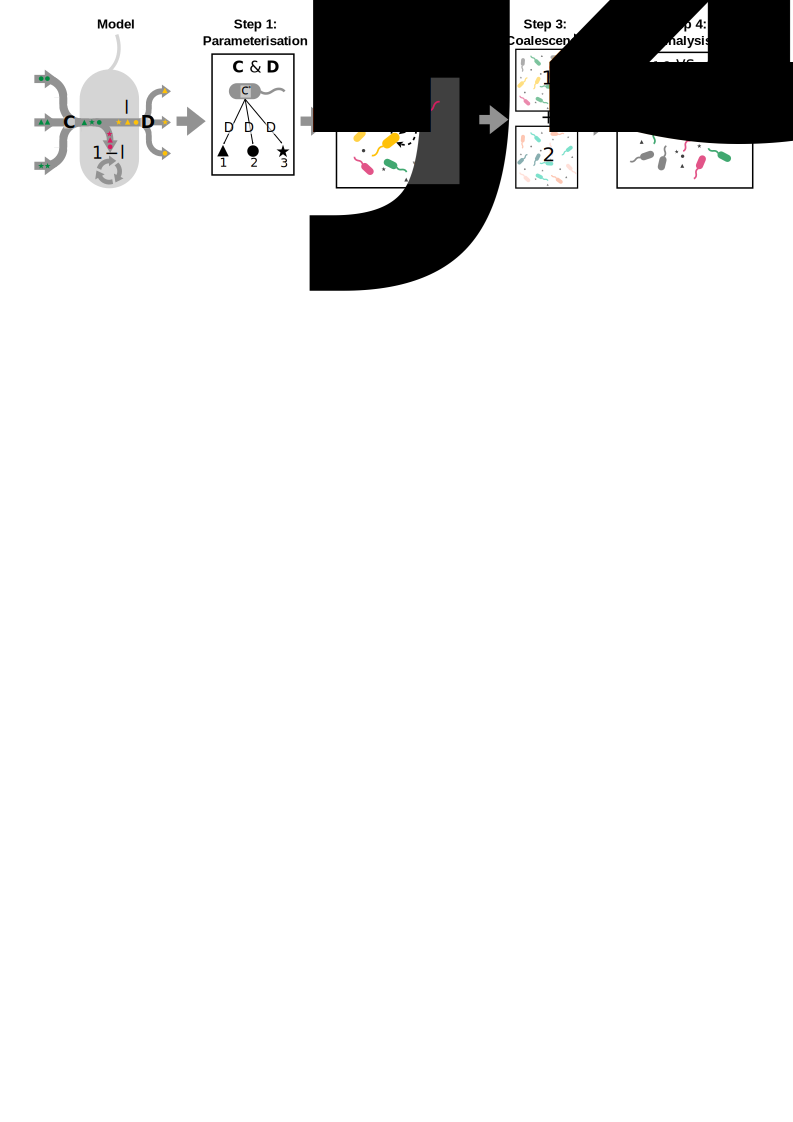
\includegraphics[width=\textwidth]{hand_plot_flow.pdf}
            \caption{\textbf{Workflow scheme.} First, the metabolic preferences of $s = 60$ bacterial strains behaving as explained in section \ref{model} and sketched in the top left corner, and one matrix $D$, are sampled for each community (parameter sampling). This sampling is done either with taxonomic and metabolic structure, or without it, as specified in section \ref{sampling}. Second, the dynamics of the sampled system play out in an environment with $m = 60$ resources, according to equations \ref{model_pop} and \ref{model_rec}, until equilibrium of the community is reached (community assembly). Third, these communities are randomly paired up and re-equilibrated together in fresh media (community coalescence). Fourth, the contribution of each community to the final mix is analyzed as a function of the competitive and facilitative interactions between species (emphasized with black arrows in the top right corner).}
            \label{work_flow}
        \end{figure}
        
        \subsection{Sampling of $ c_{{\alpha}j} $ and $ D_{jk }$ with resource demand structure}\label{sampling}
	
        	We are interested in generating communities spanning a broad range of cohesion levels, i.e., different competition and facilitation levels. These can be modified by sampling $ c_{{\alpha}j} $ and $ D_{jk} $ respectively, with specific constraints.\\
        
        	First, let us consider the problem of modulating the competition level of the community by sampling the metabolic preferences for each strain, encoded in  $ c_{{\alpha}j} $. Each species $ {\alpha} $ has a binary vector $ \vec{c_{\alpha}} $ of length $ m $ that specifies if resource $ j $ is consumed ($ c_{{\alpha}j} = 1 $) or not ($ c_{{\alpha}j} = 0 $). \\
        	The metabolic preference matrix $ C $ is constructed by sampling its rows $ \vec{c_{\alpha}} $ sequentially. The process of sampling $ \vec{c_{\alpha}} $ is two-fold. We first sample $ m_{\alpha} $, the number of metabolites that species $ {\alpha} $ consumes, from an exponential distribution. Second, to determine which metabolites are consumed by species $ {\alpha} $, we sample $ m_{\alpha} $ metabolites with probability vector $ \vec{p_{\alpha}} $. Note that in this sampling scheme, 'iteration number' and 'species' are equivalent, and denoted by index ${\alpha}$.\\
        	For species $ {\alpha} = 1 $ all metabolites have the same probability of being sampled $ 1/m $, where $ m $ is the total number of resources. This assumption is consequent with the absence of a metabolite hierarchy, since they all carry the same energy. After each iteration, the sampling probability of each metabolite changes according to what has been sampled so far. Let $ d_{{\alpha}j} $, denote the cumulative demand of resource $ j $ when the metabolic preferences of species $ {\alpha} $ are sampled. That is, the number of consumers of resource $ j $ at iteration $ {\alpha} $.
        	\begin{equation}
        		d_{{\alpha}j}  = \sum_{i = 1}^{{\alpha}}c_{ij}
        	\end{equation}
        	Based on $ d_{{\alpha}j} $, I then compute the probability that species $ {\alpha} $ is assigned resource $ j $ as one of its preferences
        	\begin{equation}\label{sampling_probability}
        		p_{{\alpha}j}= (1-k_c) \frac{1}{m}  + k_c \frac{d_{{\alpha} -1j}}{\sum_{j}d_{{\alpha}-1j}}
        	\end{equation}
        	where the denominator represents the total number of preferences sampled up until iteration $ {\alpha}-1 $, and acts as a normalization constant.\\
        	The strength with which $ p_{{\alpha}j} $ deviates from a uniform distribution is given by the parameter $ k_c \in [0, 1)$, the competitiveness factor. When $ k_c \rightarrow 1 $, competition is maximized. Thus, highly demanded metabolites are more likely to be sampled in the next iteration. On the contrary, when $ k_c = 0 $ the competition is random, since each metabolite is equally likely to be chosen. \par
        	
        	The metabolic preferences sampling procedure is implemented in the following algorithm\\[10pt]
        	\begin{algorithm}[H]
        		\SetAlgoLined
        		\For{{\alpha}  $\in\{  1, \dots, s  \}$ }{
        			Sample $ m_{\alpha} $ from an exponential distribution\\
        			Sample vector $ \vec{v} $ of $ m_{\alpha} $ integers $ \in  \{  1, \dots, m  \}$ with probability vector $ \vec{p}({\alpha}) $\\
        			Switch on sampled preferences $\vec{c_{\alpha}}[\vec{v}] = 1$ \\
        			Update $ \vec{d_{\alpha}} $\\
        			Update $ \vec{p_{\alpha}} $ using the new $ \vec{d_{\alpha}}$
        		}
        		\caption{Sampling of metabolic preferences}
        	\end{algorithm}
        	\vspace{10pt}
        	To illustrate the behaviour of the proposed sampling method, we run this algorithm for the two aforementioned values of $ k_c $ in a system with 50 metabolites and 1000 species. Overlaying the cumulative demand vector at each iteration yields representative figures of each case (see figure \ref{demand_profiles}).\\
        	\begin{figure}
        		\centering
        		\includegraphics[width=\textwidth]{kc_kf_demands.png}
        		\caption{\textbf{Sampling with structure based on resource demands.} Samples of $C$ (top) and $D$ (bottom) for different values of $k_c$ and $k_f$ respectively in a system with 60 metabolites, 60 species. Note that both constants tune the amount of structure in the matrix, so that when $k_c, k_f \rightarrow 0$ there is no structure, and when $k_c, k_f \rightarrow 1$ the structure is maximum.}
        		\label{demand_profiles}
        	\end{figure}
        
        	Second, let us consider the problem of modulating the facilitation level of the community by sampling the metabolic cross-feeding topology, encoded in the community metabolic matrix $ D $. Each element of the metabolic matrix, $ D_{jk} $, specifies the fraction of leaked energy from resource $ j $ that is released in the form of resource $ k $. Note that by definition $ \sum_jD_{jk} = 1 $.\\ 
        	The matrix element $ D_{jk} $ is constructed by adding two terms. First, the $ k^{th} $ element of a random vector following a flat Dirichlet distribution, $ \vec{x_j} \sim \text{Dir}(\vec{q})$ where all elements of the parameter vector $ \vec{q} $ are equal to one, $ q_k = 1 $. In this case, the Dirichlet distribution is equivalent to a uniform distribution over the standard ($ k  - 1 $)-simplex, where $ k \in \{1, \dots, m\} $, where $m$ is the total number of resources. The Dirichlet distribution has the property that each sampled vector sums to 1, making it a natural way of randomly allocating a fixed total quantity (such as the total secretion flux from a given input) \citep{Marsland2020}. Second, a term that depends on the difference in demand between resources $ j $ and $ k $, that is, on $ d_{sj} - d_{sk}$, where $ s $ is the number of species (omited from now on to avoid cluttering the notation). Let $ \Delta_{jk} $ denote the truncated difference between demands of resource $ j $ and $ k $ as
        	\begin{equation}
        		\Delta_{jk} = 
        			\begin{cases}
        				d_k - d_j & \text{ if } d_k > d_j\\
        				1 & \text{ if } d_k = d_j\\
        				0 & \text{ if } d_k < d_j\\
        			\end{cases}
        	\end{equation}
        	Then, the fraction of the leaked resource $ j $ that is released in the form of resource $ k $ is given by
        	\begin{equation}\label{sampling_metabolism}
        		D_{jk} = (1-k_f)x_{jk} + k_f\frac{\Delta_{jk}}{\sum_j\Delta_{jk}}
        	\end{equation}
        	The weight of each term in equation \ref{sampling_metabolism} (the uniform random term, and the resource demand dependent term) is now modulated by $ k_f \in [0, 1]$, the facilitation factor. When $ k_f = 1 $, the first term  vanishes, and facilitation is maximized. Hence, more coveted metabolites are released at higher fractions. When $ k_f = 0 $, facilitiation is uniformly random, as all metabolites are released with equiprobable fractions.\par\\
        
        	Note that although the two methods for sampling $ c $ and $ D $ share similarities, they are conceptually different. First, the sampling of $ c $ is fully random, in the sense that a vector of probabilities is constructed first, and then preferences are randomly sampled from that distribution. On the other hand, the sampling of $ D $ has a random term, $ x_{jk} $, and a non-random term that depends only on the vector of demands of the community $ \vec{d_s} $. Another difference is that the competitiveness factor is imposed on the preference sampling probability vector, while the facilitation factor is imposed directly on the values of $ D $. Finally, the sampling of $ D $ depends on the sampling of $ c $, reflecting that high or low facilitation levels are achieved by tuning the secretion structure of the community to be symmetric to the profile of demands, or independent from it, respectively.
    	
    	\subsection{Sampling $ c_{{\alpha}j} $ and $ D_{jk }$ with metabolic and taxonomic structure}
        	
        	\begin{figure}[t]
        		\centering
        		\includegraphics[width=\textwidth]{kc_kf_guilds.png}
        		\caption{\textbf{Sampling with taxonomic and metabolic structure.} Samples of $C$ (top) and $D$ (bottom) for different values of $K_c$ and $K_f$ respectively in a system with 60 metabolites, 60 species and 4 resource classes. Note that both constants tune the amount of structure in the matrix, so that when $K_c, K_f \rightarrow 0$ there is no structure, and when $K_c, K_f \rightarrow 1$ the structure is maximum.}
        		\label{kc_kf_guilds}
        	\end{figure}
            Taxonomic and metabolic structure is imposed on the  preference matrix and metabolic cross-feeding matrix, respectively, through the partition of the resource space into a set $C$ of $m_c$ resource classes.\par\\
            We define a taxonomic family $T$ as a subset of resource classes, ($T \subseteq C$), characteristic of a species. Therefore, if species $\alpha$, belongs to taxonomic family $T$ the probability of sampling resource $j$ will be higher if  that resource belongs to a resource class that is in the taxonomic family, i.e., $C(j) \in T$, and lower otherwise. The magnitude of this difference is tuned by the taxonomic heterogeneity constant $K_c \in [0, 1]$. Thus, the probability $p_{\alpha j}$ that species $\alpha$ consumes resource $j$ is given by (see section \ref{derivations} for derivation)
            \begin{equation}\label{sampling_taxonomic}
                p_{\alpha j} = 
                \begin{cases}
                    \dfrac{1}{m}\left( 1 + K_c(\dfrac{m}{n_c} - 1) \right) & \text{if } C(j) \in T  \\
                    \dfrac{1}{m}(1-K_c) & \text{otherwise}
                \end{cases}
            \end{equation}
            Note that $K_c$ controls the amount of taxonomic structure in the community. When $K_c = 1$, the probability of sampling a resource outside the taxonomic family is 0, and all the sampled preferences belong to the subset of classes conforming the taxonomic family. On the opposite end, when $K_c = 0$ the probability of sampling a resource from the taxonomic family is the same as that of sampling a resource outside the taxonomic family.\par\\
            We impose metabolic structure through a two tier secretion model. The first tier contains by-products that are not in the resource class of the substrate (off-block diagonals of $D$), and the second one contains the products that belong to the same resource class as the substrates (block diagonals of $D$). We encode this structure in $D$ by sampling each row from a Dirichlet distribution with concentration parameters $q_{jk}$ that depend on the by-product tier as:
            \begin{equation}
                D_{jk} = \text{Dir}\left(q_{j1}, q_{j2}, \dots  , q_{jm}\right)_k
            \end{equation}
            where
            \begin{equation}
                q_{jk} = 
                \begin{cases}
                    \dfrac{1-K_f}{sM_{C(j)}} & \text{if } C(j) = C(k)\\
                    \dfrac{K_f}{sM_{C(j)}} & \text{otherwise}
                \end{cases}
             \end{equation}
            Here, $s$ is the sparsity of the metabolic network, ranging from a fully connected network when $s \rightarrow 0$ to a sparse one-to-one network when $s \rightarrow 1$. $M_{C(j)}$ is the number of consumers in the class to which resource $j$ belongs. In these simulations $s = 0.05$, and the number of consumers in each class is the same $M_{C} = m/n_c$\\
            
    	\subsection{Community Assembly}
    	
        	We performed simulations of community assembly for the following parameters: $ s = 40 $, $ m = 40 $, $ k_c = [0,  \dots, 0.9]$, $ k_f = [0, \dots, 1]$, $ l = [0.05, \dots, 0.95]$. Next, I plot heat maps for each value of $ l $, of the average richness $ r $ as a function of $ k_c $ and $ k_f $. 
        	\begin{figure}[h]
        		\centering
        		\includegraphics[width=\textwidth]{kc_kf_richness.pdf}
        		\caption{Heat-maps for each value of $ l $ of the average richness $ r $ as a function of $ k_c $ and $ k_f $}
        		\label{kc_kf_richness}
        	\end{figure}
        	I find that each value of leakage represents a starkly different regime. In figure \ref{kc_kf_richness}A leakage is negligible. Average richness decreases as $ k_c $ increases, but does not change with $ k_f $. The leakage fraction is so low that the effect of the level of facilitation the diversity of the community is negligible. Figure \ref{kc_kf_richness}B represents an intermediate regime where the leakage level in the community is substantial. In this regime, the maximum average richness is reached around the top-left corner of the heat-map, where competition is lowest and facilitation is highest. Minimum average richness is reached for the opposite conditions. Figure \ref{kc_kf_richness}C illustrates communities with very high level of leakage. In this regime, highest diversity is reached by communities with low competition and facilitation levels. This result is counter intuitive, as one would expect that high facilitation promotes diversity. However, the species in  this communities are not efficient at consuming resources, since they leak the majority of what they harvest. Thus, in order to deplete the available resources, they need to perform more cycles of consumption than a species with a lower leakage factor. The optimal interaction topology that ensures efficient resource depletion in several cycles of consumption and leakage is one that minimizes facilitation and competition. \par\\
        	To sum up; predictably, the three figures show that biodiversity is favoured by niche separation, since less competitive communities are more diverse. Surprisingly, the benefit of mutualistic interactions changes for each case. When individuals are very selfish (very low $l$), mutualistic interactions are irrelevant. These become beneficial when individuals are moderately generous. However, they are detrimental, and therefore minimized when individuals are altruistic (very high $l$).
    
        \subsection{Coalescence event of two communities}\label{coalescence_event}
        
            A coalescence event in this framework is simulated by mixing the two communities that have been equilibrated independently in fresh media (the concentration of all resources is reset to that before community assembly), and letting the system relax to the a equilibrium state.\\
        
    	\subsection{Coalescence events of communities with equal $l$}
    	
    	    In the assembly process I showed that the effect of cooperation in community richness depends on the leakage level of the community. This effect is neutral when leakage is low, positive for moderate leakage, and negative for high leakage. I now turn to the question of how the community facilitation level affects the outcome of coalescence events. Is it always true that more cohesive communities perform better in coalescence events?\\
    	    To answer this question, I simulate the mixing process of two communities. Both assembled communities are introduced in a common chemostat with fresh media, and the mix is re-equilibrated. After the dynamics play out the resulting community is  This coalescence simulation is repeated many times for a broad range of leakage values. 
	
	\newpage
	
	\section{Supplementary Material}
	
	    \subsection{Equivalence with other consumer resource models}
	    
	        If we take the model equations \ref{model_pop} and \ref{model_rec} and assume that the dilution all resources is slow, that is, $ \tau_j^{-1} << 1$, in the limit when there is no leakage ($l = 0$), we can make the assumption that molecular (resource) dynamics are faster than population dynamics, and therefore that resource concentration $R_j$ at any moment quickly equilibrates to reflect the instantaneous demand thus, $ dR/dt \approx 0 $. This allows us to separate the time scales between resource and population dynamics, recovering the model presented in \cite{Tikhonov2016}\par
	        
	        \begin{equation}\label{Tikhonov_model}
		        \begin{aligned}
					\frac{dN_{\alpha}}{dt} &= g_{\alpha}N_{\alpha}\Big(\underbrace{\sum_j c_{{\alpha}j}\frac{\kappa_j}{\sum_{\alpha}N_{\alpha}c_{{\alpha}j}} - z_{\alpha}}_{\text{Resource surplus }\Delta_{\alpha}}\Big)\\
					R_j &= \frac{\kappa_j}{\sum_{\alpha}N_{\alpha}c_{{\alpha}j}}\\
		        \end{aligned}
	        \end{equation} 
        	The mapping between the notation used in \cite{Tikhonov2016} (T), \cite{Marsland2019} (M) and those used here is provided in the table:\\
	        \begin{center}
		        \begin{tabular}{ |l|c|c|c| } 
            		\hline
            		Notation for... & M & Here & T \\ 
            		\hline
            		Species index & $ i $ & $ {\alpha} $ & $\vec{\sigma}$ \\ 
            		pecies abundance & $ N_i $ & $ N_{\alpha} $ & $ n_{\sigma} $ \\ 
            		Resource a species can harvest & $ \vec{c_{i}} $ & $ \vec{c_{{\alpha}}} $ & $ \sigma_i $ \\ 
            		Resource supply & $ \kappa_{\alpha}$ & $ \kappa_j $ & $ R_i $ \\ 
            		Minimal resource requirement & $ m_i $ & $ z_{\alpha} $ & $ \chi_{\vec{\sigma}} $ \\ 
            		Resource weight & $ w_{\alpha} $ & $ \vec{1} $ & $\vec{1}$ \\ 
            		Resource $ \rightarrow $ biomass converison factor & $ g_i $ & $ g_{\alpha} $ & $ (\tau_0\chi_{\vec{\sigma}})^{-1} $ \\ 
            		Resource dilution rate & $ \tau_{\beta}^{-1} $ & $ \approx $ 0 & 0 \\ 
            		Leakage factor & $ l_{\alpha} $ & $ l $ & 0 \\ 
            		Metabolic matrix & $ D_{\alpha\beta} $ & $ D_{jk} $ & NA \\ 
            		\hline
		        \end{tabular}
	        \end{center}
	        
	    \subsection{Cost function}\label{cost_function}
	        
	        The cost function used here ensures that neither specialists or generalists are systematically favoured during community assembly, and corresponds to the assumption of approximate neutrality \citep{Tikhonov2016, Tikhonov2017, Tikhonov2018, Rosindell2012}.\\
	        Consider the surplus term in equation \ref{model_pop}. The species will increment its abundance when 
	        \begin{equation}\label{cost_harvest}
	            \frac{1}{g_{\alpha}n_{\alpha}}\frac{dn_{\alpha}}{dt} = (1-l)\sum_j c_{\alpha j}R_j - z_{\alpha} &> 0
	        \end{equation}
	        That is, species that are able to maintain positive growth for the lowest concentration of resources, will be favoured. This is can be achieved by either reducing $z_{\alpha}$ or increasing the number of resource preferences in equation \ref{cost_harvest}. However, if one imposes the constrain $z_{\alpha} = \sum_j c_{\alpha j}$, the condition to maintain positive growth becomes 
	        \begin{equation}
	            R_j - \chi_0 > 0
	        \end{equation}
	        Which is independent of the number of preferences of the consumer, that is, species are neutral under this assumption. To break this degeneracy, we introduce a small random fluctuation term ($\epsilon$ in equation \ref{cost_function}). Therefore, the cost model presented above corresponds to the assumption of approximate neutrality.\par
	        
	    \subsection{Resource recycling mechanism}\label{infinite_cycles}
	    
            The equilibrium state of the communities in these simulations is a dynamic equilibrium, because in order to maintain the biomass at steady state, the species need to harvest resources from the environment. A portion of those resources is made up by biotic resources, those leaked by the community members. These resources are also competed for in a series of consecutive cycles of consumption and leakage. When a species harvests resource $j$ from the abiotic environment, it intakes a fraction $1-l$ and leaks back a fraction $l$ in the form of other resources (first two arrows in figure \ref{cycling_scheme}). The leaked resources become part of the available substrates, and are competed for in a second cycle of consumption, with intake fraction $l(1-l)$. This process extends up to $n$ cycles, (with $n \rightarrow \infty$),  as illustrated in figure \ref{cycling_scheme}, so that at cycle $n$, the fraction of harvested resource is $l^n(1-l)$. The strength of the biotic competition and facilitation links, $B$, is calculated by summing the fraction of ingested resource over $n \in [1, \infty)$. 
            \begin{equation}
                B = \sum_{n = 1}^{\infty}\ l^n(1-l)= (1-l)\left(\sum_{n = 0}^\infty l^n -1\right) = (1-l)\left(\frac{1}{1-l} - 1\right) = l
	        \end{equation}
            \begin{figure}[t]
        		\centering
        		\includegraphics[width=0.4\textwidth]{cycling_scheme.pdf}
        		\caption{\textbf{Mechanism of resource recycling}. The species in this model consume the resources that come through the supply rate $\kappa$ (abiotic uptake, top arrow) and leak a fraction $l$ back to the environment (left arrow). The leaked resources can be harvested again by the species in the community (biotic uptake, bottom arrows). This can be modeled as an infinite series of consecutive cycles of uptake and leakage where the amount of resources consumed by each strain decreases by a factor of $l$, after each cycle.}
        		\label{cycling_scheme}
        	\end{figure}
        	As expected, the strength factor for biotic links is $l$, the fraction of substrates originally leaked. Note that this result depends on the convergence of the geometric series, which is only true when $l < 1$. In the trivial case $l = 1$, then $B = 0$, and the system would have no competitive, nor facilitative interactions.
        	
	    \subsection{Matrix representations}\label{matrix_representations}
	    
        	The implementation of this framework in Python becomes significantly more efficient if the equations are vectorized.\\
        	First, the model presented in section \ref{model} can be conveniently expressed in matrix form  as follows
        	\begin{equation}
        		\begin{aligned}
        		\frac{d\boldsymbol{n}}{dt} &= \boldsymbol{g}\circ \boldsymbol{n}\left(D(\boldsymbol{R})C(\boldsymbol{1}-\boldsymbol{l}) - \boldsymbol{z}\right)\\
        		\frac{d\boldsymbol{R}}{dt} &= \boldsymbol{\kappa} - D(\boldsymbol{R})\boldsymbol{\tau}^{\circ -1}- D(\boldsymbol{R})C^T\boldsymbol{n} + D^TD(\boldsymbol{l}\circ \boldsymbol{R})C^T\boldsymbol{n}
        		\end{aligned}
        	\end{equation}
        	where $\boldsymbol{1}$ is a column vector of ones of appropriate dimension, and $ \circ $ denotes element-wise operation\par
        	The equations presented in section \ref{metrics} can also be vectorized. In the following we use that the factor $\tilde{\kappa}_j = 1$ because in our simulations, all the resources are being supplied in the same amount. For instance, in equation \ref{abiotic}, since metabolic preferences are binary, taking the scalar product of the two preference vectors yields the number of common elements between them.
        	\begin{equation}
        	    	C_a = (1-l) CC^T
        	\end{equation}
        	For equation \ref{biotic}, only indices $j$ and $k$ can be vectorized, taking the form
        	\begin{equation}
        	    (C_b)_{\alpha \beta} = l \left(\vec{c_{\alpha}} + \vec{c_{\beta}}\right)^T D \left(\vec{c_{\alpha}}\circ \vec{c_{\beta}}\right)
        	\end{equation}
        	The vectorization of equation \ref{facilitation} is expressed as
        	\begin{equation}
        	    F = l C D C^T
        	\end{equation}
            The coalescence event presented in section \ref{coalescence_event} is simulated by mixing the species from each community after the assembly process in isolation has been completed. This can be mathematically expressed in matrix form through a system of $ s_1 + s_2 + m $ differential equations, where $ s_1 $ and $ s_2 $ are the number of species that remain in the first and second communities after their assembly, respectively. 
            \begin{equation}\label{extended_system}
        		\begin{aligned}
        		\frac{d\boldsymbol{n}_e}{dt} &= \boldsymbol{g}\circ \boldsymbol{n}_{e}\left(D(\boldsymbol{R}_e)C_{e}(\boldsymbol{1}-\boldsymbol{l}_e) - \boldsymbol{m}_e\right)\\
        		\frac{d\boldsymbol{R}}{dt} &= \boldsymbol{\kappa} - D(\boldsymbol{R})\boldsymbol{\tau}^{\circ -1}- \left[\mathbb{1} \ \mathbb{1}\right] \Big( D(\boldsymbol{R}_e)C_e^T\boldsymbol{n_e} +  D_e^TD(\boldsymbol{l_e}\circ \boldsymbol{R_e})C_e^T\boldsymbol{n}_e\Big)
        		\end{aligned}
        	\end{equation}
        	Where $ \left[\mathbb{1} \ \mathbb{1}\right] $ represents the horizontal concatenation of two $m \times m$ identity matrices. The sub-index $e$ stands for \textit{extended}. To form any of the extended vectors in equation \ref{extended_system}, one simply vertically concatenates the vectors from community 1 and community 2. Constructing an extended matrix in equation \ref{extended_system} is done by joining the two matrices alongside their diagonal. For example, constructing the vector of species abundances $\boldsymbol{n}_e$ and the metabolic matrix $D_e$ would be done as
        	\begin{equation}
        	    \boldsymbol{n}_e = \begin{bmatrix}
                                        \boldsymbol{n}^{(1)} \\
                                        \boldsymbol{n}^{(2)} \\
                                    \end{bmatrix} 
                \qquad \qquad \qquad 
                D_e = \begin{bmatrix}
                            D^{(1)} & 0 \\
                            0 & D^{(2)} \\ 
                      \end{bmatrix}
        	\end{equation}
        	where the superscripts indicate belonging to community 1 or 2
        	
	    \subsection{Preferences sampling probability with taxonomic structure}\label{derivations}
	    
            The expression for the sampling probability of each resource as a function of the resource class (equation \ref{sampling_taxonomic}) is derived as follows.\\
            We begin by assuming a higher and a lower probability depending on whether the resource class belongs is in the taxonomic family or not, and that the difference in probability is modulated by a constant $K_c$. With this two assumptions, we can write
            \begin{equation}
                p_{\alpha j} = 
                 \begin{cases}
                    \dfrac{1}{m} + a K_c & \text{if } C(j) \in T  \\[10pt]
                    \dfrac{1}{m} - b K_c & \text{otherwise}
                 \end{cases}
             \end{equation}
            Now we impose that (1) the sum of the elements of $\vec{p_{\alpha}}$ must equal to 1, and (2) the lower probability must be 0 when $K_c = 1$. These constrains yield the following systems of equations that can be solved for $a$ and $b$.
            \begin{equation}
                \begin{cases}
                    n_c\left(\dfrac{1}{m} + a K_c\right) + (m-n_c)\left(\dfrac{1}{m} - b K_c\right) = 1 \\
                    \frac{1}{m} - b = 0
                \end{cases}
            \end{equation}
            Finding that 
            \begin{equation}
                a = \frac{1}{n_c} - \frac{1}{m} \qquad \text{and } \qquad b = \frac{1}{m}
            \end{equation}
            and obtaining equation \ref{sampling_taxonomic}
            
        \subsection{Table of parameter values}\label{parameter_values}
        Table of parameter values!
	\newpage
	\bibliographystyle{agsm}
	\bibliography{references}

\end{document}